% This is "aamas2016_sample.tex", a revised version of aamas2015_sample.tex
% This file should be compiled with "aamas2016.cls"
% This example file demonstrates the use of the 'aamas2015.cls'
% LaTeX2e document class file. It is intended for those submitting
% articles to the AAMAS-2016 conference. This file is based on
% the sig-alternate.tex example file.
% The 'sig-alternate.cls' file of ACM will produce a similar-looking,
% albeit, 'tighter' paper resulting in, invariably, fewer pages
% than the original ACM style.
%
% ----------------------------------------------------------------------------------------------------------------
% This .tex file (and associated .cls ) produces:
%       1) The Permission Statement
%       2) The Conference (location) Info information
%       3) The Copyright Line with AAMAS data
%       4) NO page numbers
%
% as against the acm_proc_article-sp.cls file which
% DOES NOT produce 1) through 3) above.
%
% Using 'aamas2015.cls' you don't have control
% from within the source .tex file, over both the CopyrightYear
% (defaulted to 20XX) and the IFAAMAS Copyright Data
% (defaulted to X-XXXXX-XX-X/XX/XX).
% These information will be overwritten by fixed AAMAS 2015  information
% in the style files - it is NOT as you are used to with ACM style files.
%
% ---------------------------------------------------------------------------------------------------------------
% This .tex source is an example which *does* use
% the .bib file (from which the .bbl file is produced).
% REMEMBER HOWEVER: After having produced the .bbl file,
% and prior to final submission, you *NEED* to 'insert'
% your .bbl file into your source .tex file so as to provide
% ONE 'self-contained' source file.
%

\RequirePackage{snapshot} %%% Delete Me!!!!!!!!!!!!!!!!!!!!!!!!!!!!!!!!!!!!!!!!!!!!!!!!!!!!!!!!!!!!!!!!!!!!!!!!!!!!!!!!!!!!!!!!!!!1

\documentclass{aamas2016}

\graphicspath{{img/}}

% if you are using PDF LaTeX and you cannot find a way for producing
% letter, the following explicit settings may help

\pdfpagewidth=8.5truein
\pdfpageheight=11truein

\begin{document}

% In the original styles from ACM, you would have needed to
% add meta-info here. This is not necessary for AAMAS 2015  as
% the complete copyright information is generated by the cls-files.


\title{A Multi-Domain Trust Framework for Autonomous Mobile Networks in Harsh Environments}

% AUTHORS


% For initial submission, do not give author names, but the
% tracking number, instead, as the review process is blind.

% You need the command \numberofauthors to handle the 'placement
% and alignment' of the authors beneath the title.
%
% For aesthetic reasons, we recommend 'three authors at a time'
% i.e. three 'name/affiliation blocks' be placed beneath the title.
%
% NOTE: You are NOT restricted in how many 'rows' of
% "name/affiliations" may appear. We just ask that you restrict
% the number of 'columns' to three.
%
% Because of the available 'opening page real-estate'
% we ask you to refrain from putting more than six authors
% (two rows with three columns) beneath the article title.
% More than six makes the first-page appear very cluttered indeed.
%
% Use the \alignauthor commands to handle the names
% and affiliations for an 'aesthetic maximum' of six authors.
% Add names, affiliations, addresses for
% the seventh etc. author(s) as the argument for the
% \additionalauthors command.
% These 'additional authors' will be output/set for you
% without further effort on your part as the last section in
% the body of your article BEFORE References or any Appendices.

%\numberofauthors{8} %  in this sample file, there are a *total*
% of EIGHT authors. SIX appear on the 'first-page' (for formatting
% reasons) and the remaining two appear in the \additionalauthors section.
%

\numberofauthors{1}

\author{
% You can go ahead and credit any number of authors here,
% e.g. one 'row of three' or two rows (consisting of one row of three
% and a second row of one, two or three).
%
% The command \alignauthor (no curly braces needed) should
% precede each author name, affiliation/snail-mail address and
% e-mail address. Additionally, tag each line of
% affiliation/address with \affaddr, and tag the
% e-mail address with \email.
% 1st. author
%\alignauthor
%Andrew Bolster\\
%       \affaddr{Department of Electrical Engineering and Electronics}\\
%       \affaddr{University of Liverpool}\\
%       \affaddr{United Kingdom}\\
%       \email{andrew.bolster@liv.ac.uk}
%% 2nd. author
%\alignauthor
%Alan Marshall\\
%       \affaddr{Department of Electrical Engineering and Electronics}\\
%       \affaddr{University of Liverpool}\\
%       \affaddr{United Kingdom}\\
%       \email{alan.marshall@liv.ac.uk}
%% 3rd. author
%\alignauthor Lars Th{\o}rv{\"a}ld\titlenote{This author is the one who did all the really hard work.}\\
%       \affaddr{The Th{\o}rv{\"a}ld Group}\\
%       \affaddr{1 Th{\o}rv{\"a}ld Circle}\\
%       \affaddr{Hekla, Iceland}\\
%       \email{larst@affiliation.org}
Registration ID\#176
}

%\and  % use '\and' if you need 'another row' of author names

% 4th. author
%\alignauthor Lawrence P. Leipuner\\
%       \affaddr{Brookhaven Laboratories}\\
%       \affaddr{Brookhaven National Lab}\\
%       \affaddr{P.O. Box 5000}\\
%       \email{lleipuner@researchlabs.org}

% 5th. author
%\alignauthor Sean Fogarty\\
%       \affaddr{NASA Ames Research Center}\\
%       \affaddr{Moffett Field}\\
%       \affaddr{California 94035}\\
%       \email{fogartys@amesres.org}

% 6th. author
%\alignauthor Charles Palmer\\
%       \affaddr{Palmer Research Laboratories}\\
%      \affaddr{8600 Datapoint Drive}\\
%       \affaddr{San Antonio, Texas 78229}\\
%       \email{cpalmer@prl.com}

%\and

%% 7th. author
%\alignauthor Lawrence P. Leipuner\\
%       \affaddr{Brookhaven Laboratories}\\
%       \affaddr{Brookhaven National Lab}\\
%       \affaddr{P.O. Box 5000}\\
%       \email{lleipuner@researchlabs.org}

%% 8th. author
%\alignauthor Sean Fogarty\\
%       \affaddr{NASA Ames Research Center}\\
%       \affaddr{Moffett Field}\\
%       \affaddr{California 94035}\\
%       \email{fogartys@amesres.org}

%% 9th. author
%\alignauthor Charles Palmer\\
%       \affaddr{Palmer Research Laboratories}\\
%       \affaddr{8600 Datapoint Drive}\\
%       \affaddr{San Antonio, Texas 78229}\\
%       \email{cpalmer@prl.com}

%}

%% There's nothing stopping you putting the seventh, eighth, etc.
%% author on the opening page (as the 'third row') but we ask,
%% for aesthetic reasons that you place these 'additional authors'
%% in the \additional authors block, viz.
%\additionalauthors{Additional authors: John Smith (The Th{\o}rv{\"a}ld Group,
%email: {\texttt{jsmith@affiliation.org}}) and Julius P.~Kumquat
%(The Kumquat Consortium, email: {\texttt{jpkumquat@consortium.net}}).}
%\date{30 July 1999}
%% Just remember to make sure that the TOTAL number of authors
%% is the number that will appear on the first page PLUS the
%% number that will appear in the \additionalauthors section.

\maketitle

\begin{abstract}

Trust Management Frameworks (TMFs) are being used to improve the efficiency, security, and reliability of decentralized and distributed autonomous systems. 
Techniques have been developed for high-speed, uncontended environments such as terrestrial 802.11 MANETs. 
However, these do not perform well in sparse / harsh environments such as those found in Underwater Acoustic Networks (UANs), where network nodes experience significant and variable delays, comparatively low data rates, large contention periods, and considerable multi-path artefacts.\cite{Bolster2015} 

In such sparse networks, trust establishment based on statistical observations of success/failure events become unstable and ineffective in detecting or identifying misbehaviours. 
Additionally, these methodologies focus solely on the communications activities of entities and do not incorporate information from other domains, such as physical mobility. 

In this paper we demonstrate the use and operation of a multi-domain trust management framework (MD-TMF) using UANs as an exemplar application. 
%We demonstrate a methodology that applies Grey Sequence operations and Grey Generators (conceptually analogous to Sequential Bayesian Filtering) to provide continuous trust assessment in a sparse, asynchronous metric space across multiple domains of trust.
We present a preliminary methodology for assessing the performance of varying metric sets in detection and differentiation of a range of communications and physical misbehaviours, demonstrating that by utilising information from multiple domains, trust assessment can be more accurate in identifying misbehaviour than in single-domain assessment.


\end{abstract}

% Note that the category section should be completed after reference to the ACM Computing Classification Scheme available at
% http://www.acm.org/about/class/1998/.

\category{H.4}{Information Systems Applications}{Miscellaneous}

%A category including the fourth, optional field follows...
%\category{D.2.8}{Software Engineering}{Metrics}[complexity measures, performance measures]

%General terms should be selected from the following 16 terms: Algorithms, Management, Measurement, Documentation, Performance, Design, Economics, Reliability, Experimentation, Security, Human Factors, Standardization, Languages, Theory, Legal Aspects, Verification.

\terms{Algorithms Management Performance Reliability Security}

%Keywords are your own choice of terms you would like the paper to be indexed by.

\keywords{MANET, Underwater, Simulation, Trust}

\section{Introduction}
With the increasing integration of autonomy into modern cyber-physical systems, Trust Management Frameworks (TMFs) are being applied to safeguard the efficiency, security, and reliability of decentralised and distributed networks of autonomous systems, from highway-bound autonomous vehicles to aerial battlefield drones. 
Classical implementations of trust management in Mobile Ad-Hoc Networks (MANETs) have focused solely on observations from the communications domain to make trust assessments. 
However, these methods are not as effective in applications exhibiting sparse, delayed, or otherwise challenged communications environments\cite{Pavan2015}. 

In the majority of Trusted MANET implementations, a free space RF communications protocol such as 802.11 is used.
By their nature, such implementations rely on relatively high bandwidth, low noise, low latency, high channel occupancy where contention is tolerable.
In contrast; in underwater environments, communications is sparse, delayful, noisy, and very prone to destructive contention.
Therefore the observations about the communications processes that are used to generate the trust metrics, occur much less frequently, with much greater error (noise) and delay than is experienced in terrestrial RF MANETS.
In addition to the communications challenges, other considerations such as command and control isolation, as well as power and locomotive limitations, drive towards the use of teams of smaller, cheaper, almost disposable autonomous underwater vehicles (AUVs), particularly in defense, ecological and petrochemical fields.
. These increasingly decentralised applications present unique threats against trust management. 

Trust Management Frameworks (TMFs) provide information to assist the estimation of future states and actions of nodes within networks. This information is used to optimize the performance of a network against malicious, selfish, or defective misbehaviour by one or more nodes. Previous research has established the advantages of implementing TMFs in 802.11 based MANETs, particularly in terms of preventing selfish operation in collaborative systems \cite{Li2007}, and maintaining throughput in the presence of malicious actors \cite{Buchegger2002}. Most current TMFs use a single type of observed action to derive trust values, typically successfully delivered or forwarded packets. These observations then inform future decisions of individual nodes, for example, route selection \cite{Li2008}.

Recent work has demonstrated the use of a number of metrics to form a ``vector'' of trust. The Multi-parameter Trust Framework for MANETs (MTFM) \cite{Guo11}, uses a range of communications metrics beyond packet delivery/loss rate (PLR) to assess trust. This vectorized trust also allows a system to detect and identify the tactics being used to undermine or subvert trust. This method as been previously applied to the marine space, comparing against a selection of existing communications TMFs \cite{Bolster2015} showing that MTFM is more effective at detecting misbehaviours in sparse environments. This paper builds upon that work to encompass physical as well as communications observations in the establishment of trust and the detection and classification of misbehaviours across both physical and communications domains. 
An example area of application is the underwater marine environment, where extreme challenges to communications are present (propagation delays, frequency dependent attenuation, fast and slow fading, refractive multi-path distortion, etc.).
\begin{figure}[h!]
	\centering
	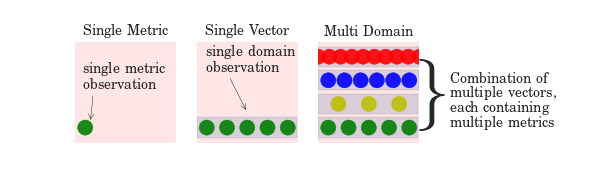
\includegraphics[width=\linewidth]{threat_surface_sum}
	
	\caption{The inclusion of additional metrics and domains in trust assessment reduces the systems exposed threat surface}
\end{figure}

This paper is laid out as follows; in Section 2 we discuss Trust and TMFs, defining out terminology and reviewing the justifications for the use and development of TMFs in harsh environments such as UANs.
In Section 3 we review selected features of the underwater communications channel, highlighting particular challenges against terrestrial equivalents. 
In Section 4 we review the findings of \cite{Bolster2015} and establish experimental parameters and simulated behaviours under assessment. 
In Section 5 we present our analysis method for assessing misbehaviour using MTFM, and intermediate results of the independent detection of physical and communications misbehaviours using single-domain observations. 
In Section 6 we demonstrate results from multi-domain MTFM and discuss the significance of these findings in terms of detection and classification of cross-domain misbehaviour sets.

\section{Trust Management Frameworks}

\subsection{Trust in Connected Systems}

For a term that is so common in every-day speech, Trust is a challenging discussion area, particularly given the wealth of proposed definitions \cite{Lee2004}. Beyond these often ``fuzzy'' definitions, there is a significant ontological conflict between the subjective and objective perspectives of trust; is ``trust'' an attribute of the actor performing a given action, or of the observer of such an action? Or indeed is trust itself an action upon a relationship between actors? Is it qualitative or quantitative? These questions have challenged philosophers, psychologists and social scientists for decades.

In human trust relationships it is recognized that there can be several domains of Trust for example organizational, sociological, interpersonal, psychological and neurological \cite{Lee2004}.

In the context of trust between and among collectives of autonomous systems, it is the quantifiable assessment of the expected reliability of an entity to perform a given task on request by another entity. This trust assessment can be targeted towards the reliability of a single task or as a general indicator of ``trustworthiness'' of a range of activities.

In many systems, this ``trust'' is analogous to ``security'', and these terms are often conflated, however in this case we are not necessarily concerned with the security of a system so much as it's runtime reliability in operation.

Within networked systems, the aspect of operation that usually need to be protected from malicious operation or failure states most is bandwidth and congestion, i.e. optimising the network to maximum energy/time efficiency for transiting information.
In this respect, the Router Information Protocols (RIP) can be considered very basic Trust Management Frameworks, such that they optimise routing structures within a network based on (binary) link availability.\cite{RFC2453}.

However, in more complex systems and application, communications optimality is not necessarily the only aspect of operation under threat.
Particularly in Mobile Ad-Hoc Networks, individual node constraints such as energy supply and any other consumables present another exploitable vector for attack.
Further, in applications such as persistent survey and observation, operational considerations such as the end-to-end delay in reporting or the reduction in the timely observed area may be threatened by misbehaviour.


\subsection{Trust in Conventional MANETs}
The distributed and dynamic nature of MANETs mean that it is difficult to maintain a trusted third party (TTP) systems or evidence based trust system such as Certificate Authorities (CA) or Public Key Infrastructure (PKI). 
Distributed trust management frameworks aim to detect, identify, and mitigate the impacts of malicious actors by distributing per-node assessments and opinions to collectively police behaviour. 

Various models and algorithms for describing trust and developing trust management in distributed systems, P2P communities or wireless networks have been considered.
\textit{Hermes Trust Establishment Framework} uses a Bayesian Beta function to model per-link Packet Loss Rate (PLR) over time, combining ``Trust'' and ``Confidence of Assessment'' into a single value \cite{Zouridaki2005}.
\textit{Objective Trust Management Framework} (OTMF) builds upon Hermes and distributes node observations across the network \cite{Li2008}, however does not appropriately combat multi-node-collusion in the network \cite{Cho2011}. 
\textit{Trust-based Secure Routing} demonstrated an extension to Dynamic Source Routing (DSR), incorporating a Hidden Markov Model of sub-networks, reducing the efficacy of Byzantine attacks such as black-hole routing  \cite{Moe2008a}. 
\textit{CONFIDANT} presented an approach using a probabilistic estimation of PLR, similar to OTMF, also introducing a topology aware weighting scheme and also weighting trust assessments based on historical experience of the reporter \cite{Buchegger2002}. Fuzzy Trust-Based Filtering uses Fuzzy Inference to adapt to malicious recommenders using conditional similarity to classify performance with overlapping fuzzy set membership, filtering assessments across a network \cite{Luo2008}.
\textit{Multi-parameter Trust Framework for MANETs} (MTFM) uses a number of communications metrics together for form a vector of trust, apply grey information theory to allow a system to detect and identify the tactics being used to undermine or subvert trust\cite{Guo11}.

These TMFs (excluding MTFM) can be generalised as single-value estimation based on a binary input state (success or failure of packet delivery) and generating a probabilistic estimation of the future states of that input (how likely is it that the next transmission will reach it's destination?). 
These single metric TMFs provide malicious actors with a significant advantage if their activity does not impact that metric.
In the case where the attacker can subvert the TMF, the metric under assessment by that TMF does not cover the threat mounted by the attacker. 
This causes a significant negative effect on the efficiency of the network, as the TMF is assumed to have reduced the possible set of attacks when it has actually made it more advantageous to attack a different part of the networks operation.
An example of such a situation would be in a TMF focused on PLR where an attacker selectively delays packets going through it, reducing overall throughput but not dropping any packets. Such behaviour would not be detected by the TMF.

As an example; The Hermes trust establishment framework \cite{Zouridaki2005} uses Bayesian reasoning to generate a posterior distribution function of ``belief'', or trust, given a sequence of observations of that behaviour, $p(B|O)$\eqref{eq:otmf_pbo}.

\begin{equation}
p(B|O)  = \frac{p(O|B) \times p(B)}{\rho}
\label{eq:otmf_pbo}
\end{equation}

Where $p(B)$ is the prior probability density function for the expected normal behaviour, and $\rho$ is a normalising factor.
Due to it's flexibility and simplicity, Hermes assumes that $p(B)$ is a Beta function, and therefore the evaluation of this trust assessment is based around the expectation value of the distribution \eqref{eq:otmf_t}  where $\alpha$ and $\beta$ represent the number of successful and unsuccessful interactions respectively for a particular node $i$.

A secondary measurement of the confidence factor of the trust assessment $t$ is generated as \eqref{eq:otmf_c} and these measurements are combined to form a ``trustworthiness'' value $T$ \eqref{eq:otmf_trust}.

\begin{align}
t_i &\to E\lbrack\text{beta}(p|\alpha,\beta)\rbrack = \frac{\alpha_i}{\alpha_i+\beta_i} \label{eq:otmf_t}\\[5pt]
c_i &= 1 - \sqrt{\frac{12\alpha_i\beta_i}{(\alpha_i+\beta_i)^2(\alpha_i+\beta_i+1)}} \label{eq:otmf_c}\\[5pt]
T_i &= 1 - \frac{\sqrt{\frac{(t_i-1)^2}{x^2} + \frac{(c_i-1)^2}{y^2}}}{\sqrt{\frac{1}{x^2}+\frac{1}{y^2}}} \label{eq:otmf_trust}
\end{align}

In \eqref{eq:otmf_trust}, $x$ and $y$ are constants, used weight the two-dimensional polar mapping of trust and confidence assessments ($t_i,c_i$), and from \cite{Zouridaki2005}, are taken as $x=\sqrt{2},y=\sqrt{9}$.

Upon this per-node assessment methodology, OTMF overlays an observation distribution protocol so as to make the measurements $\alpha_i$ and $\beta_i$ representative of the direct and 1-hop networks observations of the target node $i$, as well as expiring old observations from assessment and eliminating observations from ``untrustworthy'' nodes.


\textit{Multi-Parameter Trust Framework for MANETS} (MTFM) extends this single-parameter approach, applying Grey Relational Analysis \cite{Zuo1995} to provide cohort based normalization of a range of disparate metrics at runtime, providing a ``grade'' of trust compared to other observed nodes, while maintaining the ability to reduce trust valued down to a stable assessment range for decision support without requiring a-priori environmental or metric characterisation. This presents a stark difference between the previously discussed probabilistic approaches. Grey assessments are relative in both fairly and unfairly operating networks. All nodes will receive mid-range trust assessments if there are no malicious actors as there is nothing ``bad'' to compare against, and variations in assessment will be primarily driven by topological and environmental factors.

Guo et al. \cite{Guo11} demonstrated the ability of grey relational analysis (GRA) \cite{Zuo1995} to normalise and combine disparate traits of a communications link such as instantaneous throughput, received signal strength, etc. into a grey relational coefficient (GRC), or a ``trust vector'' in this instance.

The grey relational vector is given as
%
\begin{align}
\label{eq:grc}
\theta_{k,j}^t = \frac{\min_k|a_{k,j}^t - g_j^t| + \rho \max_k|a_{k,j}^t-g_j^t|}{|a_{k,j}^t-g_j^t| + \rho \max_k|a_{k,j}^t-g_j^t|} \\
\phi_{k,j}^t = \frac{\min_k|a_{k,j}^t - b_j^t| + \rho \max_k|a_{k,j}^t-b_j^t|}{|a_{k,j}^t-b_j^t| + \rho \max_k|a_{k,j}^t-b_j^t|} \notag 
\end{align}
%
where $a_{k,j}^t$ is the value of an observed metric $x_j$ for a given node $k$ at time $t$, $\rho$ is a distinguishing coefficient set to $0.5$, $g$ and $b$ are respectively the ``good'' and ``bad'' reference metric sequences from $\{a_{k,j}^t k=1,2\dots K\}$, normally $g_j=\max_k({a_{k,j}^t})$,  $b_j=\min_k({a_{k,j}^t})$ where each metric is monotonically positive for trust assessment. 

Weighting can be applied before generating a scalar value \eqref{eq:metric_weighting} allowing the detection and classification of misbehaviours.

%
\begin{equation}
\label{eq:metric_weighting}
[\theta_k^t, \phi_k^t] = \left[\sum_{j=0}^M h_j \theta_{k,j}^t,\sum_{j=0}^M h_j \phi_{k,j}^t \right]
\end{equation}
%
Where $H=[h_0\dots h_M]$ is a metric weighting vector such that $\sum h_j = 1$, and in unweighted case, $H=[\frac{1}{M},\frac{1}{M}\dots\frac{1}{M}]$.
$\theta$ and $\phi$ are then scaled to $[0,1]$ using the mapping $y = 1.5 x - 0.5$.
To minimise the uncertainties of belonging to either best ($g$) or worst ($b$) sequences in \eqref{eq:grc} the $[\theta,\phi]$ values are reduced into a scalar trust value by $T_k^t = ({1+{(\phi_k^t)^2}/{(\theta_k^t)^2}})^{-1}$ \cite{Hong2010}.
MTFM combines this GRA with a topology-aware weighting scheme \eqref{eq:networkeffects} and a fuzzy whitenization model \eqref{eq:whitenization}. 

There are three classes of topological trust relationship used; Direct, Recommendation, and Indirect.
Where an observing node $n_i$ assesses the trust of another target node, $n_j$; the Direct relationship is $n_i$'s own observations $n_j$'s behaviour.
In the Recommendation case, a node $n_k$ which shares Direct relationships with both $n_i$ and $n_j$, gives its assessment of $n_j$ to $n_i$.
In the Indirect case, similar to the Recommendation case, the recommender $n_k$ does not have a direct link with the observer $n_i$ but $n_k$ has a Direct link with the target node, $n_j$.
These relationships give node sets, $N_R$ and $N_I$ containing the nodes that have recommendation or indirect, relationships to the observing node respectively.
%
\begin{align}
\label{eq:networkeffects}
T_{i,j}^{MTFM}=&\frac{1}{2} \cdot \max_s\{f_s(T_{i,j})\} T_{i,j}\\ \notag
+&\frac{1}{2} \frac{2|N_R| }{2|N_R| + |N_I|}\sum_{n \in N_R} \max_s\{f_s(T_{i,n})\} T_{i,n}\\ \notag
+&\frac{1}{2} \frac{|N_I| }{2|N_R| + |N_I|}\sum_{n \in N_I} \max_s\{f_s(T_{i,n})\} T_{i,n} 
\end{align}

Where $T_{i,n}$ is the subjective trust assessment of $n_i$ by $n_n$, and $f_s = [ f_1,f_2, f_3]$ given as:

\begin{align}
\label{eq:whitenization}
f_1(x)&= -x+1\notag\\
f_2(x)&= 
\begin{cases}
2x & \text{if }x\leq 0.5\\
-2x+2 & \text{if }x>0.5
\end{cases}\\
f_3(x)&= x\notag
\end{align}
%
In the case of the terrestrial communications network used in \cite{Guo11}, the observed metric set $X = {x_1,\dots,x_M}$ representing the measurements taken by each node of its neighbours at least interval, is defined as $X=[$packet loss rate, signal strength, data rate, delay, throughput$]$.

Guo et al. demonstrated that when compared against OTMF and Hermes trust assessment in terrestrial 802.11 based MANETs, MTFM provided increased variation in trust assessment over time, providing more information about the nodes' behaviours than packet delivery probability alone can.
By weighting the metrics used in MTFM it was shown that the trust assessments could be used to identify the style of misbehaviour being performed within the network, and by whom.
It has been demonstrated that MTFM is a strong candidate for trust assessment in the harsh marine communications environment \cite{Bolster2015}.

\subsection{Multi-Metric Single Domain Trust in Harsh Environments}

It has been demonstrated that classical, single metric, MANET Trust Management Frameworks are not directly suitable to the sparse, noisy, and dynamic underwater medium, however MTFM shows promise in it's multi-metric normalisation approach when compared to the performance of OTMF and Hermes in the same scenarios \cite{Bolster2015}.
In a simulated underwater environment, MTFM was able to discriminate between communications behaviours using communications metrics by exploring the metric space by weight variation, allowing the detection and classification of the malicious behaviours.
With significant end-to-end delays (from seconds to many minutes), in a fading, refractive medium with varying propagation characteristics, the environment is not as predictable or performant as classical MANET TMF deployment environments. 
Without significant adaptation, single metric probabilistic estimation based TMFs are ineffective in such an environment. This is because existing frameworks are overly optimistic about the nature and stability of the communications channel, and can overlook characteristics that are useful for assessing the behaviour of nodes in the network. 
This indicates that there is a good case for bringing together information from the commmunications and physical domains together to assess and monitor trustworthiess, particularly within constrained MANETs as in the underwater acoustic realm.


\section{Marine Acoustic Communications}

The key challenges of underwater acoustic communications are centred around the impact of slow and differential propagation of energy (RF, Optical, Acoustic) through water, and its interfaces with the seabed / air.
The resultant difficulties include; long propagation delays, significant inter-symbol interference and Doppler spreading, fast and slow fading due to environmental effects (aquatic flora/fauna, surface weather), carrier-frequency dependent signal attenuation, multi-path caused by reflective medium interfaces, variations in propagation speed due to depth dependant effects (salinity, temperature, and pressure), and subsequent refractive spreading and lensing due to that same propagation variation \cite{Partan2006}.

The attenuation that occurs in an underwater acoustic channel over a distance $d$ for a signal about frequency $f$ in linear power is given as $A_{\text{aco}}(d,f) = A_0d^ka(f)^d$ and in $dB$ form as;
%
\begin{equation}
\label{eq:acoattenuationdb}
10 \log A_{\text{aco}}(d,f)/A_0 = k \cdot 10 \log d + d \cdot 10 \log a(f)
\end{equation}
%
where $A_0$ is a normalising constant, $k$ is a spreading factor (commonly taken as 1.5  \cite{Stojanovic2007}), and $a(f)$ is the absorption coefficient, approximated using Thorp's formula \cite{Stefanov2011}
%
\begin{equation}
\label{eq:thorp}
10 \log a(f) = \frac{0.11 \cdot f^2}{1+f^2} + \frac{44\cdot f^2}{4100+f^2}+ 2.75\times10^{-4} f^2 + 0.003
\end{equation}
%

Refractive lensing and the multi-path nature of the medium result in line of sight propagation being extremely unreliable for estimating distances to targets.
The first arriving acoustic signal has as the very least curved in the medium, and commonly has reflected off the surface/seabed before arriving at a receiver, creating secondary paths that are sometimes many times longer than the first arrival path, generating symbol spreading over orders of seconds depending on the ranges and depths involved.
Forward Error Correction coding is used on such channels to minimise packet losses.

Comparing $A_{aco}(d,f)$ with the RF Free-Space Path Loss model $(A_{\text{RF}}(d,f) \approx \left( \frac{4\pi d f}{c} \right)^2)$, the impact of range on signal power is exponential underwater, rather than quadratic in terrestrial RF ($A_{\text{aco}} \propto f^{2d}$ vs $A_{\text{RF}} \propto (df)^2$). 
While both frequency dependant factors are quadratic, approximating the factors in \eqref{eq:thorp}, $f\propto A_{\text{aco}}$ is at least 4 orders of magnitude higher than $f\propto A_{\text{RF}}$


\section{Analysis, Design and Per-Domain Results}

\subsection{Simulation and Scenario Generation}
To investigate the operation of a fully mobile network of six nodes, each kinematically modelled on the commonly used REMUS100 AUV platform \cite{Milgram2001} in the marine environment, simulations were conducted using a Python based framework, SimPy \cite{Mueller2003SimPy}, with a network stack built upon AUVNetSim \cite{Miquel2008}, using transmission parameters (Table \ref{tab:sysconstraints}) taken from and validated against \cite{Stojanovic2007} and \cite{Stefanov2011}.

Four scenarios were developed to assess both communications and physical domains where one node within the fleet was 'misbehaving' ($n_m$). In cases where $n_m$ is specifically targeting another node in the fleet, that node is denoted as $n_t$.

\begin{enumerate}
	\item Malicious Power Control (MPC), where $n_m$ increases its transmit and forwarding power by 20\% for all nodes \emph{except} communications from $n_t$ in order to make $n_t$ appear to be selfishly conserving energy to the rest of the team, while $n_t$ itself appears to be performing very well.
	\item Selfish Target Selection (STS), where $n_m$ preferentially communicates, forwards and advertises to nodes that it estimates are physically close to it in effort to reduce its own power consumption.
	\item Shadowing, where $n_m$ is not aware of the pre-planned mission paths and is instead simply following it's neighbours.
	\item Slow Coach, where $n_m$ is experiencing a simulated power-train failure that reduces it's acceleration and top speed, analogous to a fouled propeller. 
\end{enumerate}

The default scenario is also simulated where nodes participate fairly in the network and follow a collaborative survey mobility pattern.

From these simulations, we attain the per-node recorded positions, ($P_i = [x,y,z] \forall t$) as well as each nodes estimations of it's neighbours positions $P_{i,j} = [x,y,z] \forall t$) (which assumes that all nodes are fairly reporting their positions compactly at each transmission), and each nodes trust metric observations of it's neighbours; $A_{i,j}^t = [ x_{i,j} \forall x \in X ] $ where $X$ are the selected trust metrics.

%
\begin{table}[h]
	\caption{System model constraints} \label{tab:sysconstraints}
	\begin{center}
		\setlength{\tabcolsep}{8pt}
		\begin{tabular}{lccc}
			\hline
			Parameter & Unit & Value \\
			\hline
			Simulated Duration & $s$ & 18000\\
			Initial Separation & $m$ & 300\\
			Trust Sampling Period & $s$ & 600 \\
			Simulated Area & $km^2$ &  0.7-4 \\
			Transmission Range & $km$ & 1.5 \\
			Physical Layer & Acoustic\\
			Propagation Speed& $m/s$ & 1490\\
			Center Frequency& $Hz$ & $2 \times 10^4$ \\
			Bandwidth& $Hz$ & $1\times10^4$\\
			MAC Type & & CSMA/CA\\
			Routing Protocol & & FBR \\
			Max Speed & $ms^{-1}$ & 1.5 \\
			Max Data Rate & $bps$ & $\approx 240$ \\
			Packet Size & bits &  9600 \\
			Single Message Duration & $s$ & 32 \\
			Single Message Size & bits & $9600$ \\
			\hline
		\end{tabular}
		\setlength{\tabcolsep}{6pt}
	\end{center}
\end{table}
%

\subsection{Communications Trust Metrics}

We use the same trust metrics from \cite{Guo2012} that are applicable to the marine environment, i.e. as the simulated modem stack does not operate on the same tiered data-rate approach as used in the 802.11 stack, that metric was not included. Remaining metrics are; Delay, Received and Transmitted power, Received and Transmitted Throughput, and Packet Loss Rate (PLR).

Thus, the metric vector used for communications-trust assessment is;

\begin{equation}
	X_{comms}=\{D, P_{RX}, P_{TX}, Tp_{RX}, Tp_{TX}, PLR\}
	\label{eq:comms_vector}
\end{equation}

\subsection{Physical Trust Metrics}

Three physical metrics are selected to encompass the relative distributions and activities of nodes within the network; Inter-Node Distance Deviation (INDD), Inter-Node Heading Deviation (INHD), and Node Speed. These metrics encapsulate the relative distributions of position and velocity within the fleet, optimising for the detection of outlying or deviant behaviour within the fleet.

Conceptually, INDD is a measure of the average spacing of an observed node with respect to its neighbours. INHD is a similar approach with respect to node orientation.

\begin{align}
	INDD_{i,j} &= \frac{|P_j - \sum_x \frac{P_x}{N}|}{\frac{1}{N}\sum_x \sum_y{|P_x - P_y| (\forall x \neq y)}}\\
	INHD_{i,j} &= \hat{v} \vert v= V_j - \sum_x{\frac{V_x}{N}}\\
	S_{i,j} &= |V_j|
\end{align}

Thus, the metric vector used for physical-trust assessment is;

\begin{equation}
  X_{phy}=\{\text{INDD}, \text{INHD}, S\}
	\label{eq:phys:vector}
\end{equation}

\subsection{Metric Weight Analysis Scheme}

From \eqref{eq:metric_weighting}, the final trust values arrived at are dependent on metric values, the weights assigned to each metric, and the structure of the $g$, $b$ comparison vectors.

This permits the assessment of the significance of different metrics in the detection and identification of different behaviours. 
For a metric weight vector $H$, where the metric $m_j$ is emphasised as being twice as important as the other metrics, we form an initial weighting vector $H'=[h_i...h_M]$ such that $h_i = 1 \forall i \ne j; h_j=2$. We then scale that vector $H'$ such that $\sum H = 1$ by $H= \frac{H'}{\sum H'}$.

The construction of the $g$ and $b$ vectors from \ref{eq:grc} depends on the particular metric, e.g. Throughput is positively correlated to trustworthiness and so follows the default construction ($g \mapsto \max, b \mapsto \min$).
However, in the case of a metric such as delay, this relationship is inverted, i.e. longer delays indicate less trustworthy activity.
In complex environments, the relationship between metrics trustworthiness correlations may not be quite so obvious as the throughput / delay examples.
This phenomenon was mentioned by Guo, but was manually configured for each metric for each behaviour and no analytical method for quantatively establishing such relationships has been presented since.

We include both the correlation and relevance of metrics to behaviours by signifying ``flipped'' metrics (i.e. those with the construction $g \mapsto \min, b \mapsto \max$) by a negative weight.

Using this process we can extract and highlight the primary aspects of an attack by comparing against the deviation from the ``fair'' result set, i.e. we are interested in the weight schemes that create the largest difference between fair and misbehaving cases.

With the nine selected metrics from across communications and physical behaviours, we can explore this metric space by varying the weights associated with each metric, and choose to emphasise across three levels; i.e. metrics can be ignored or over-emphasised. Naively this results in $3^9 = 19683$ combinations, however as these weights are being normalised, duplicates are introduced, e.g. $[0,0,0,0,1,0,0,0,0] \equiv [0,0,0,0,2,0,0,0,0]$ leaving 18661 unique weights for analysis.

To assess the performance of a given weight combination (i.e. an optimisation factor), we are initially interested in the metric weight vector that consistently provides the largest deviation in the final trust value $T$ across the cohort, i.e. producing the most clear detection of a node misbehaving in that particular fashion.
We approach this as an inverse outlier filtering problem, and select the range outside a $\pm\sigma$ envelope compared to the equivalent weighting in a known ``fair'' behaviour to assess detection (or comparing to other misbehaviours to assess discrimination). Note that at this point we establish ``signatures'' of different behaviours rather than optimal detection weights.

We apply a Random Forest regression \cite{Breiman2001} to assess the relative importance of the selected metrics on relative detectability of malicious behaviour. 
Random Forest accomplishes this by generating a large number of random regression trees and prune these trees to fit incoming data. A major advantage of Random Forest in this case is that by walking the most successful regression trees, we can acquire an already normalised maximal activation weight for the particular behaviour comparison being tested.

After establishing the importance of weights in particular behaviours, a final weight is arrived at by algorithmically those few metrics that are important, rather than having to further explore the computationally expensive weight-space.

Using this approach we can explore the results of these simulations, condensing the multi-dimensional problem (target / observer / behaviour / metric / time) down to a more tangible level for analysis.

\section{Results and Discussion}

\subsection{Significance Analysis}

First we discuss the results of the Random Forest regression assessment; in Figs~\ref{fig:comms_feature_extraction} and ~\ref{fig:phys_feature_extraction}, we show the resultant feature extraction signatures for Comms-only and Physical-only metric selections, and Fig~\ref{fig:multi_feature_extraction}, these metric spaces are brought together and reassessed.

It is also interesting to note that in both single-domain cases, there are clear 'signatures' in misbehaviours that don't directly target that domain ($P_{RX}$ in the Physical Shadow and Slowcoach behaviours in Fig~\ref{fig:comms_feature_extraction} and $INDD$ in the Selfish Target Selection behaviour in Fig~\ref{fig:phys_feature_extraction}).
This inter-domain activity is to be expected in MANETs in general, where the physical reality of the network (i.e. distance between nodes) directly impacts the behaviour of the logical communications network (i.e. delay between nodes), and is as we will see a useful characteristic for differentiating potential misbehaviours.



\begin{figure}[h!]
	\centering
  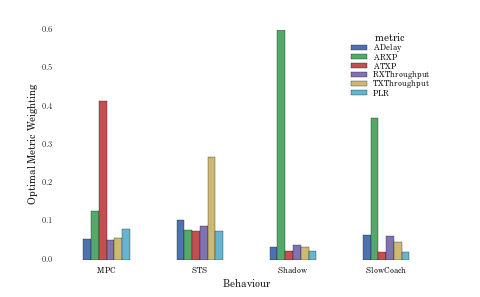
\includegraphics[width=\linewidth]{comms_metric_trust_relevance}
	\caption{Plot of $X_{comms}$ Metric Feature Extraction}
	\label{fig:comms_feature_extraction}
\end{figure}

\begin{figure}[h!]
	\centering
  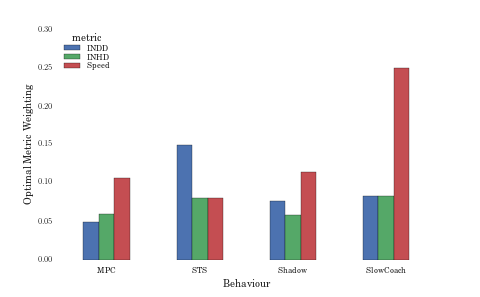
\includegraphics[width=\linewidth]{phys_metric_trust_relevance}
	\caption{Plot of $X_{phys}$ Metric Feature Extraction}
	\label{fig:phys_feature_extraction}
\end{figure}

\begin{figure}[h!]
  \centering
  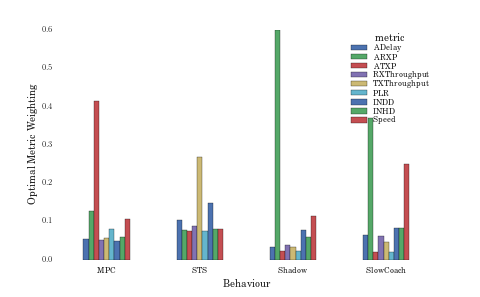
\includegraphics[width=\linewidth]{full_metric_trust_relevance}
  \caption{Multi Domain Relevance assessment of Metric Features}
  \label{fig:multi_feature_extraction}
\end{figure}

%\begin{tabular}{lrrrrrrrrr}
\toprule
{} &  $Delay$ &  $P_{RX}$ &  $P_{TX}$ &  $T^P_{RX}$ &  $PLR$ &  $T^P_{TX}$ &  $INDD$ &  $INHD$ &  $Speed$ \\
Misbehaviour &          &           &           &             &        &             &         &         &          \\
\midrule
MPC          &   -0.187 &     0.129 &     0.579 &       0.006 &  0.069 &      -0.146 &   0.040 &  -0.190 &   -0.297 \\
STS          &   -0.195 &    -0.035 &     0.019 &      -0.100 &  0.019 &       0.381 &  -0.209 &   0.057 &    0.062 \\
Shadow       &    0.004 &    -0.654 &     0.030 &      -0.016 &  0.030 &       0.063 &   0.120 &   0.158 &    0.266 \\
SlowCoach    &   -0.157 &    -0.533 &     0.013 &      -0.132 &  0.013 &      -0.028 &   0.159 &   0.206 &    0.460 \\
\bottomrule
\end{tabular}


\subsection{Weight Assessment}

From this significance information we can infer a signature for each behaviour, that can be fed back into the assessment framework, with the aim being to minimise the number of weight permutations required to come to a conclusion about the behaviour under observation. 

We take the feature significances as presented from the regression as baseline weight vectors, however, we have no algorithmically derived approach to the structure of the $g$,$b$ comparison vectors from \eqref{eq:metric_weighting}.

One option would be to go back to the regression point and expand the combination options to include negative values, however this is combinatorically explosive.
Instead, the ``significance'' weight is permuted against it's possible combinations of ``flips'', i.e. for $X_s=[0.3,0.4,0.01,0.02,0.27]$ could also be $X_s^p=[0.3,-0.4,0.01,0.02,0.27]$ and so on. 
This sign permutation is filtered based on a threshold value ($0.01$), so for all indices below that threshold will not be permuted on, halving the number of combinations required for each indices eliminated.

The best of these permutations is selected to both maximise the (correct) deviation between each nodes trust perspectives and to minimise the trust value reported for the misbehaving nodes; $\Delta T \max$

These weights are applied to untrained data to derive the following results.

An exemplar subset of the results is shows in Figs~\ref{fig:comms_sts}-\ref{fig:full_slowcoach}, with the "misbehaving node" highlighted with heavier lines, with any observations about the rest of the cohort faded and dashed. For each node assessment, the mean for that assessment over that time period is also included as a solid / dashed line respectively for clarity.

Comparing Figs~\ref{fig:comms_sts} and \ref{fig:full_sts}, while there is a reasonable dip in the misbehavor's trust assment, the variance across the cohort is such that this "mistrust" triggering is neither consistent or obvious. Unfortunately this is the case across the STS responses, where in Table~\ref{tab:domain_deltas} where we have summarized out general results, STS has by far and away the lowest average $\Delta T$ in all domains. Interestingly however is the observation that Comms-only trust performs slightly better than Full trust weighting.

Referring to Figs~\ref{fig:comms_feature_extraction} and \ref{fig:multi_feature_extraction}, it's clear that the transmitted throughput ($T^P_{TX}$) is the almost singular feature of this behaviour, due to it's almost completly logical behaviour that is only loosely coupled to the state of the environment. 
The massive emphasis placed on throughput could only be diminished by putting it together in a larger ensemble.

The other "Primary Communications" behaviour, MPC, is not shown for brevity, but scores comfortably in the 90th percentile range in both full and comms trust assessments.

In Figs~\ref{fig:comms_shadow} and \ref{fig:full_shadow}, the misbehaving node is much more obvious than in STS, which is moderatly surprising for a physically-focused behaviour. Further, there is a roughly 20\% improvement when incorporating the full metric space.

From Table~\ref{tab:domain_deltas}, the Shadow behavior is the most consistently detectible behaviour across domains. 

\begin{figure}[h]
	\centering
	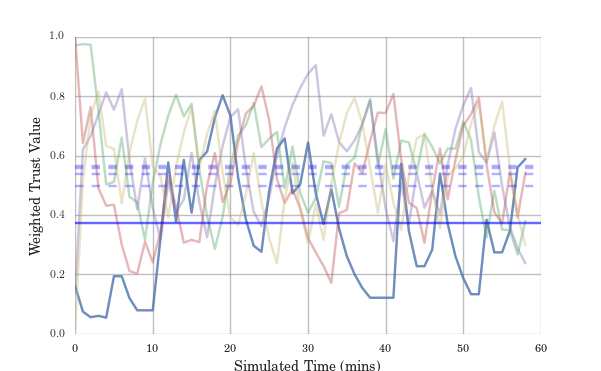
\includegraphics[width=\linewidth]{best_comms_run_STS}
	\caption{Selfish(STS) Targeting Comms Metric Trust}
	\label{fig:comms_sts}
\end{figure}

\begin{figure}[h]
	\centering
	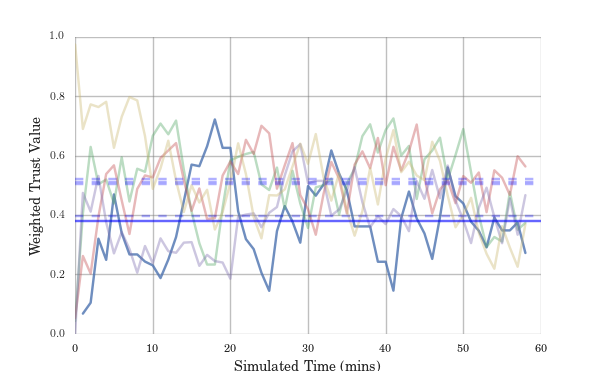
\includegraphics[width=\linewidth]{best_full_run_STS}
	\caption{Selfish(STS) Targeting Full Metric Trust}
	\label{fig:full_sts}
\end{figure}

\begin{figure}[h]
	\centering
	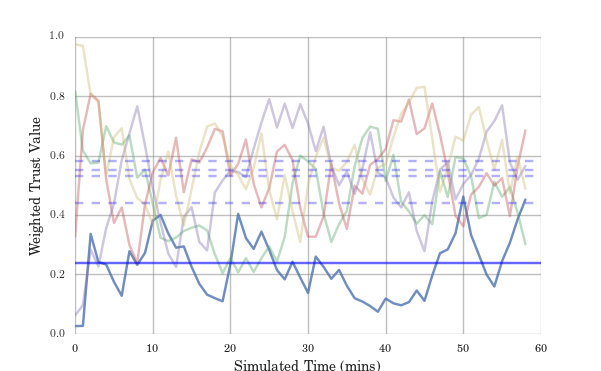
\includegraphics[width=\linewidth]{best_comms_run_Shadow}
	\caption{Shadow Comms Metric Trust}
	\label{fig:comms_shadow}
\end{figure}

\begin{figure}[h]
	\centering
	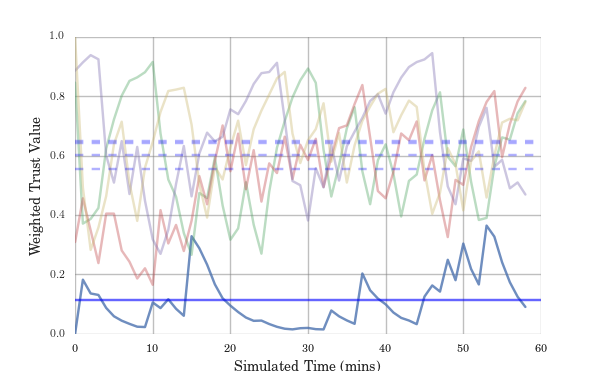
\includegraphics[width=\linewidth]{best_full_run_Shadow}
	\caption{Shadow Full Metric Trust}
	\label{fig:full_shadow}
\end{figure}


\begin{figure}[h]
	\centering
  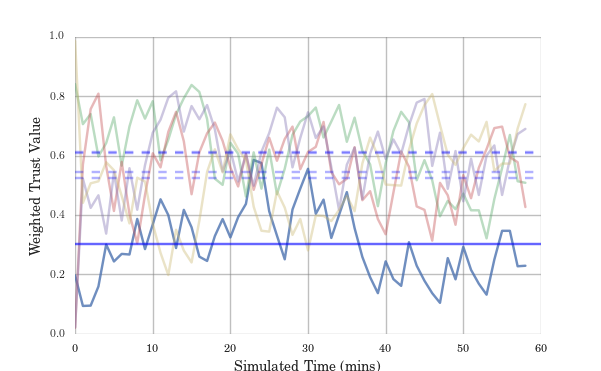
\includegraphics[width=\linewidth]{best_comms_run_SlowCoach}
	\caption{SlowCoach Comms Metric Trust}
	\label{fig:comms_slowcoach}
\end{figure}


\begin{figure}[h]
	\centering
  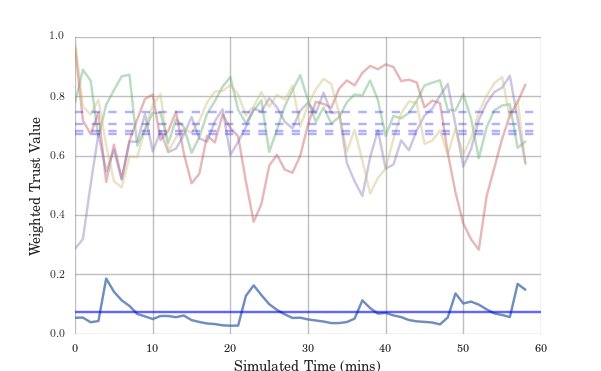
\includegraphics[width=\linewidth]{best_full_run_SlowCoach}
	\caption{SlowCoach Full Metric Trust}
	\label{fig:full_slowcoach}
\end{figure}


\begin{table}
\centering
\caption{$\Delta T$ across domains and detected behaviours}
\begin{tabular}{|l|r|r|r|r|r|}
\hline
Behaviour &       MPC &       STS &    Shadow & SlowCoach & Avg.\\
\hline
Domain &           &           &           &           &\\
Full   &  0.905 &  0.101 &  0.499 &  0.627 & 0.533\\
Comms  &  0.954 &  0.166 &  0.287 &  0.268 & 0.419 \\
Phys   &  0.022 &  0.020 &  0.421 &  0.756 & 0.305\\
\hline
Avg.   &  0.627 &  0.096 &  0.402 &  0.550 &  0.419 \\
\hline
\end{tabular}
\label{tab:domain_deltas}
\end{table}

\section{Conclusion}
In this paper we demonstrate that in harsh environments, multi-domain trust assessment can perform better on average than single-domain counterparts, both in terms of robustness and sensitivity, but also covering a wider region of the potential behaviour space, 

The extension of the methodologies of multi-vector trust into the marine space are already demonstrated, however including information from physical observations of actors in a network enables the detection and identification of a much wider range of behaviours.
We also demonstrate a method for assessing trust metrics in harsh environments in terms of their relative significance, and a method for establishing classification signatures for misbehaviours.

It is to be noted that this presented method is significantly more computationally intensive than the relatively simple Hermes / OTMF algorithms communications only algorithms, and is exponential in complexity as metrics and/or domains are added. The repeated metric re-weighting required for real time behaviour detection is therefore an area that requires optimization. More work needs to be done to characterise how worthwhile this approach is compared to a separate synthesis approach where by MTFM-style trust is generated and assessed on a per-domain basis and subsequently fuzed.

For greater fidelity and more optimal results, a wider range of weights can be used in the initial regression step; however this is computationally expensive given that weighting is applied to each perspective (i.e. observer/target node pair) for each trust assessment time step, presenting 15 perspectives at each time interval in the 6 node case.

Every effort has been made to avoid over-training the dataset, using cross validating sampling for regression and "best weight" generation, however more meta-analysis is required to further demonstrate the functionality of this process.


% For AAMAS-2016, as references are unlimited but appendices must fit within
% 8 pages, the References section must come after the appendices (if any)
%
% The following two commands are all you need in the
% initial runs of your .tex file to
% produce the bibliography for the citations in your paper.
\bibliographystyle{abbrv}
\bibliography{refs}  % sigproc.bib is the name of the Bibliography in this case
% You must have a proper ".bib" file
%  and remember to run:
% latex bibtex latex latex
% to resolve all references
%
% ACM needs 'a single self-contained file'!
%\balancecolumns % GM June 2007
% That's all folks!
\end{document}
